\documentclass{exam}

\usepackage{indentfirst}
\usepackage{graphicx}
\usepackage{listings}
\usepackage{color}
\usepackage{fancyvrb}
\usepackage{amsmath}

\definecolor{mygreen}{rgb}{0,0.6,0}
\definecolor{mygray}{rgb}{0.5,0.5,0.5}
\definecolor{mymauve}{rgb}{0.58,0,0.82}

\lstset{ %
	backgroundcolor=\color{white},		% choose the background color; you must add \usepackage{color} or \usepackage{xcolor}
	basicstyle=\small\ttfamily,		% the size of the fonts that are used for the code
	breakatwhitespace=false,			% sets if automatic breaks should only happen at whitespace
	breaklines=true,					% sets automatic line breaking
	captionpos=b,						% sets the caption-position to bottom
	columns=fullflexible,
	commentstyle=\color{mygreen},		% comment style
	deletekeywords={...},				% if you want to delete keywords from the given language
	escapeinside={\%*}{*)},			% if you want to add LaTeX within your code
	extendedchars=true,				% lets you use non-ASCII characters; for 8-bits encodings only, does not work with UTF-8
	frame=single,						% adds a frame around the code
	keepspaces=true,					% keeps spaces in text, useful for keeping indentation of code (possibly needs columns=flexible)
	keywordstyle=\color{blue},			% keyword style
	language=Octave,					% the language of the code
	morekeywords={*,...},				% if you want to add more keywords to the set
	%   numbers=left,						% where to put the line-numbers; possible values are (none, left, right)
	%   numbersep=6pt,						% how far the line-numbers are from the code
	%   numberstyle=\tiny\color{mygray},	% the style that is used for the line-numbers
	rulecolor=\color{black},			% if not set, the frame-color may be changed on line-breaks within not-black text (e.g. comments (green here))
	showspaces=false,					% show spaces everywhere adding particular underscores; it overrides 'showstringspaces'
	showstringspaces=false,			% underline spaces within strings only
	showtabs=false,					% show tabs within strings adding particular underscores
	stepnumber=1,						% the step between two line-numbers. If it's 1, each line will be numbered
	stringstyle=\color{mymauve},		% string literal style
	tabsize=2,							% sets default tabsize to 2 spaces
	title=\lstname						% show the filename of files included with \lstinputlisting; also try caption instead of title
}

\newcommand{\octavescript}[2]{
	\lstinputlisting[caption=#2,label=#1]{#1}
}

\newcommand{\MNLab}{Laborator\ \#9}
\newcommand{\MNLabTitle}{Metoda Neville. Metode de interpolare cu funcţii spline cubice. Curbe B\'{e}zier. Algoritmul De Casteljau}
\newcommand{\MNLabTitleHeader}{Interpolare}
\newcommand{\MNAuthor}{Andrei STAN, Dumitru-Clementin Cercel, Bogdan Marchiș}

\renewcommand{\contentsname}{Cuprins}
\renewcommand{\figurename}{Figura}

\setlength{\parskip}{0.5\baselineskip}

\graphicspath{{./img/}}

\title{
	\textmd{\textbf{\MNLabTitle}}
	\author{Colaboratori: \MNAuthor}
}

\pagestyle{headandfoot}

\header{Metode Numerice}
{\MNLabTitleHeader, Pagina \thepage\ din \numpages}
{2025}
\footer{Facultatea de Automatică și Calculatoare}{}{Pagina \thepage\ din \numpages}

\begin{document}

\begin{coverpages}

	\maketitle
	\tableofcontents

\end{coverpages}

\section{Obiective laborator}

În urma parcurgerii acestui laborator, studentul va fi capabil să:
\begin{itemize}
	\item calculeze valoarea unei funcţii într-un punct folosind metoda Neville;
	\item aproximeze traiectoria unei funcţii cu ajutorul funcţiilor spline cubice;
	\item traseze o curba B\'{e}zier folosind algoritmul De Casteljau.
\end{itemize}

\section{Noțiuni teoretice}

\subsection{Metoda Neville}

Se consideră o funcţie $f:[a, b] \rightarrow R$ cunoscută într-o mulţime finită de puncte $x_0,x_1, ...,x_n$ (numite suportul interpolării) prin valorile: $$f(x_0), f(x_1), ...,f(x_n).$$

Metoda Neville este o metodă de interpolare care aproximează comportamentul funcţiei $f$ în afara acestor $n+1$ puncte. În cele ce urmează, folosim notaţia $P_{ij}(x)$ pentru a reprezenta polinomul de interpolare de grad $j-i$ care trece prin punctele $(x_l, f(x_{l})), l=i, i+1,...,j$.

Polinomul de interpolare $P_{ij}$ este dat de relaţie de recurentă:
$$P_{ij}(x) = \frac{x-x_j}{x_i-x_j}P_{i,j-1}(x) + \frac{x_i-x}{x_i-x_j}P_{i+1,j}(x), \quad 0 \leq i < j \leq n $$

\noindent unde
$$P_{ii}(x)=f(x_{i}), \quad i = 0:n.$$

În prima iteraţie, metoda Neville construieşte polinoame de interpolare de grad 0, reprezentatate prin $P_{ii}(x), i = 0:n$. În următoarea iteraţie, oricare două polinoame de interpolare de grad 0, alăturate, $P_{ii}$ şi $P_{i+1, i+1}, i=0:n-1$, formează un polinom de interpolare de grad 1 notat cu $P_{i, i+1}(x)$. Procesul continuă până când se obţine polinomul de interpolare $P_{0, n}$ care trece prin toate cele $n+1$ puncte $(x_l, f(x_{l})), l=0,...,n$. De exemplu, procesul iterativ de obţinere al polinomului de interpolare $P_{03}(x)$, pentru $n=3$, este arătat în schema următoare:

\begin{center}
	\begin{tabular}{ccccccc}
		$P_{00}(x)=f(x_0)$ & {}          & {}                                                                  \\
		{}                 & $\searrow $ & {}          & {}                                                    \\
		{}                 & {}          & $P_{01}(x)$ & {}                                                    \\
		{}                 & $\nearrow $ & {}          & $\searrow $                                           \\
		$P_{11}(x)=f(x_1)$ & {}          & {}          & {}          & $P_{02}(x)$                             \\
		{}                 & $\searrow $ & {}          & $\nearrow $ & {}          & $\searrow $               \\
		{}                 & {}          & $P_{12}(x)$ & {}          & {}          & {}          & $P_{03}(x)$ \\
		{}                 & $\nearrow $ & {}          & $\searrow $ & {}          & $\nearrow$                \\
		$P_{22}(x)=f(x_2)$ & {}          & {}          & {}          & $P_{13}(x)$                             \\
		{}                 & $\searrow $ & {}          & $\nearrow $                                           \\
		{}                 & {}          & $P_{23}(x)$ & {}                                                    \\
		{}                 & $\nearrow $ & {}                                                                  \\
		$P_{33}(x)=f(x_3)$ & {}          & {}          & {}                                                    \\
	\end{tabular}
\end{center}

%%%%%%%%%%%%%%%%%%%%%%%%%%%%%%%%%%%%%%%%%%%%%%%%%%%
\subsection{Metode de interpolare cu funcţii spline cubice}

În continuare, considerăm că funcţia $f:[a, b] \rightarrow R$ este cunoscută atât într-o mulţime finită de puncte $x_0,x_1, ...,x_n$ prin valorile: $$f(x_0), f(x_1), ...,f(x_n)$$
cât şi prin derivatele de ordin I ale funcţie în aceste puncte:
$$f^{'}(x_0), f{'}(x_1), ...,f{'}(x_n)$$

În cazul interpolării cu funcţii spline cubice, comportamentul funcţiei $f$ se va studia local pe subintervalele:
$$[x_0,x_1), [x_1,x_2), ...,[x_i,x_{i+1})..., [x_{n-1},x_{n})$$

Astfel, pentru fiecare subinterval $[x_i,x_{i+1})$ se va considera o funcţie de interpolare de gradul 3 (numită funcţie spline cubică) de forma:$$s_i:[x_i,x_{i+1}) \rightarrow R,
	s_i(x) = a_i + b_i(x-x_i) + c_i(x-x_i)^2 + d_i(x-x_i)^3$$

Prin schimbarea de variabilă $t= \frac{x-x_i}{x_{i+1}-x_i}$ se obţine următoarea formă parametrică pentru o funcţie spline cubică:
$$s_i(t) = a_i + b_i h_i t + c_i h_i t^2 + d_i h_i t^3$$

\noindent unde am notat $h_i = x_{i+1}-x_i$.

În general, se foloseşte baza de interpolare Bernstein pentru a eficientiza procesul de calculare al coeficienţilor funcţiilor spline cubice:
$$(1-t)^3,3t(1-t)^2,3t^2(1-t),t^3$$

Folosind baza de interpolare Bernstein, funcţia spline cubică devine		:
$$s_i(t) = a_i^{'} (1-t)^3 + 3b_i^{'}t(1-t)^2 + 3c_i^{'}t^2(1-t) + d_i^{'}t^3$$

\subsubsection{Interpolare cu funcţii spline în clasa $C^1$:}
Pentru a determina cei $4n$ coeficienţi, se impun următorele condiţii în cazul interpolării cu funcţii spline în clasă $C^1$:\begin{itemize}
	\item $2n+2$ condiţii de interpolare de tip Hermite:
	      \begin{center}
		      $s_i(x_i) = f(x_i), \quad i = 0:n-1$
	      \end{center}
	      \begin{center}
		      $s_{n-1}(x_n) = f(x_n)$
	      \end{center}
	      \begin{center}
		      ${s_{i}}^{'}(x_i) = f^{'}(x_i), \quad i = 0:n-1$
	      \end{center}
	      \begin{center}
		      ${s^{'}_{n-1}}(x_n) = f^{'}(x_n)$
	      \end{center}

	\item $2n-2$ condiţii de racordare ce asigură continuitatea şi derivabilitatea funcţiilor spline cubice vecine:
	      \begin{center}
		      $s_i(x_{i+1}) = s_{i+1}(x_{i+1}), \quad i = 0:n-2$
	      \end{center}
	      \begin{center}
		      ${s_i}^{'}(x_{i+1}) = {s^{'}_{i+1}}(x_{i+1}), \quad i = 0:n-2$
	      \end{center}
\end{itemize}

În rezolvarea sistemului format din cele $4n$ ecuaţii, considerăm pentru funcţiile spline cubice forma parametrică în baza Bernstein. Se obţin următoarele relaţii pentru coeficienţi:
$$a_i^{'} = f(x_{i}), \quad i = 0:n-1$$
$$d_i^{'} = f(x_{i+1}), \quad i = 0:n-1$$
$$b_i^{'} = f(x_{i})+\frac{h_i}{3}f^{'}(x_i), \quad i = 0:n-1$$
$$c_i^{'} = f(x_{i+1})-\frac{h_i}{3}f^{'}(x_{i+1}), \quad  i = 0:n-1$$

\noindent iar forma parametrică pentru funcţiile spline cubice în baza Bernstein devine:
$$s_i(t) =  f(x_{i})(1-t)^3 + [3 f(x_{i})+h_i f^{'}(x_{i})]t(1-t)^2  +[3 f(x_{i+1}) - h_i f^{'}(x_{i+1})]t^2(1-t) +
	f(x_{i+1})t^3$$

În cele din urmă, se poate obţine forma în variabila $x$ pentru fiecare funcţie spline cubică în clasă $C^1$ prin schimbarea de variabilă
$t= \frac{x-x_i}{h_i}$.

\subsubsection{Interpolare cu funcţii spline în clasă $C^2$:}

În cazul interpolării cu funcţii spline în clasă $C^2$, cei $4n$ coeficienţi se determină prin impunerea a:

\begin{itemize}
	\item $n+1$ condiţii de interpolare de tip Lagrange:
	      \begin{center}
		      $s_i(x_i) = f(x_i), \quad i = 0:n-1$
	      \end{center}
	      \begin{center}
		      $s_{n-1}(x_n) = f(x_n)$
	      \end{center}

	\item $3n-3$ condiţii de continuitate, derivabilitate şi curbură pentru funcţiile spline cubice vecine:
	      \begin{center}
		      $s_i(x_{i+1}) = s_{i+1}(x_{i+1}), \quad i = 0:n-2$
	      \end{center}
	      \begin{center}
		      ${s_i}^{'}(x_{i+1}) = {s^{'}_{i+1}}(x_{i+1}), \quad i = 0:n-2$
	      \end{center}
	      \begin{center}
		      ${s_i}^{''}(x_{i+1}) = {s^{''}_{i+1}}(x_{i+1}), \quad i = 0:n-2$
	      \end{center}

	\item următoarelor 2 condiţii pentru funcţiile spline naturale:
	      \begin{center}
		      ${s_0}^{''}(x_{0}) = 0$
	      \end{center}
	      \begin{center}
		      ${s^{''}_{n-1}}(x_{n})=0$
	      \end{center}

	      respectiv următoarelor 2 condiţi pentru funcţiile spline tensionate:
	      \begin{center}
		      ${s_0}^{'}(x_{0}) = {f}^{'}(x_{0})$
	      \end{center}
	      \begin{center}
		      ${s^{'}_{n-1}}(x_{n}) = {f}^{'}(x_{n})$
	      \end{center}
\end{itemize}

În cele ce urmează, se consideră pentru fiecare funcţie spline cubică forma în variabiala $x$. Coeficienţii funcţiilor spline cubice în clasă $C^2$ sunt daţi de relaţiile:
$$a_i = f(x_{i}), \quad i = 0:n$$
$$d_i = \frac {c_{i+1}-c_i}{3h_i}, \quad i = 0:n-1$$
$$b_i = \frac {a_{i+1}-a_i}{h_i} - \frac {h_i}{3} (2c_i+c_{i+1}), \quad i = 0:n-1$$

\noindent iar coeficienţii $c_i, i = 0:n-1$ se obţin prin rezolvarea unui sistem tridiagonal de forma:

- pentru funcţii spline naturale
\begin{equation*}
	\begin{bmatrix}
		{1}   & {0}          & {0}       & {   }                & { 0 }     \\
		{h_0} & {2(h_0+h_1)} & {h_1}     & {   }                & {0 }      \\
		{   } & \ddots       & \ddots    & \ddots               & { }       \\
		{   } & { }          & {h_{n-2}} & {2(h_{n-2}+h_{n-1})} & {h_{n-1}} \\
		{ 0 } & {   }        & { }       & {0}                  & {1}       \\
	\end{bmatrix}
	\begin{bmatrix}
		{c_0 }     \\
		{c_1 }     \\
		\vdots     \\
		{c_{n-1} } \\
		{c_n }     \\
	\end{bmatrix}
	=
	\begin{bmatrix}
		{0}                                                                     \\
		\frac {3(a_2-a_1)}{h_1} - \frac {3(a_1-a_0)}{h_0}                       \\
		\vdots                                                                  \\
		\frac {3(a_{n}-a_{n-1})}{h_{n-1}} - \frac {3(a_{n-1}-a_{n-2})}{h_{n-2}} \\
		{0}                                                                     \\
	\end{bmatrix}
\end{equation*}

- pentru funcţii spline tensionate
\begin{equation*}
	\begin{bmatrix}
		{2h_0} & {h_0}        & {0}       & {   }                & { 0 }      \\
		{h_0}  & {2(h_0+h_1)} & {h_1}     & {   }                & {0 }       \\
		{   }  & \ddots       & \ddots    & \ddots               & { }        \\
		{   }  & { }          & {h_{n-2}} & {2(h_{n-2}+h_{n-1})} & {h_{n-1}}  \\
		{ 0 }  & {   }        & { }       & {h_{n-1}}            & {2h_{n-1}} \\
	\end{bmatrix}
	\begin{bmatrix}
		{c_0 }     \\
		{c_1 }     \\
		\vdots     \\
		{c_{n-1} } \\
		{c_n }     \\
	\end{bmatrix}
	=
	\begin{bmatrix}
		\frac {3(a_1-a_0)}{h_0} - 3f^{'}(x_0)                                   \\
		\frac {3(a_2-a_1)}{h_1} - \frac {3(a_1-a_0)}{h_0}                       \\
		\vdots                                                                  \\
		\frac {3(a_{n}-a_{n-1})}{h_{n-1}} - \frac {3(a_{n-1}-a_{n-2})}{h_{n-2}} \\
		3f^{'}(x_n) - \frac {3(a_n - a_{n-1})}{h_{n-1}}                         \\
	\end{bmatrix}
\end{equation*}

Funcţia spline $s_n$ a fost introdusă pentru a ajuta la calcularea funcţiilor spline $s_i, i=0:n-1$.

\subsection{Curbe B\'{e}zier}
Fiind dată o mulţime de $n+1$ puncte $P_0,P_1,...,P_n$ (numite \textit{puncte de control}) în plan sau în spaţiu, curba B\'{e}zier de grad $n$ determinată de aceste puncte are forma parametrică:
$$B(t) = \sum\limits_{i=0}^n P_iB_{i,n}(t), \quad t\in[0,1]$$

\noindent unde $B_{i,n}(t)$ se numesc polinoame Bernstein de grad $n$ definite prin relaţia:
$$B_{i,n}(t) = {n \choose i} (1-t)^{(n-i)}t^i, \quad i=0:n $$

Gradul polinomului care aproximează curba Bezier depinde de numărul punctelor de control. Fiecare punct de control afectează forma curbei B\'{e}zier în mod particular. Dacă modificăm poziţia unui punct de control şi forma curbei B\'{e}zier va fi afectată.

Spre deosebire de funcţiile spline, curba B\'{e}zier nu trece prin fiecare punct de control. Orice curbă B\'{e}zier începe în punctul de control $P_0$ şi se termină în punctul de control $P_n$ adică:
$$B(0) = P_0, B(1) = P_n$$

Mai mult, curba B\'{e}zier este tangentă segmentelor $P_0P_1$ si $P_{n-1}P_n$ adică:
$$B^{'}(0) = n(B_1-B_0), B^{'}(1) = n(B_n-B_{n-1})$$

O altă proprietate este aceea că orice curbă B\'{e}zier este conţinută complet de înfăşurătoarea convexă pe care punctele de control o definesc.

În mod uzual, se folosesc curbe B\'{e}zier cubice determinate de 4 puncte de control, având forma parametrică:

\begin{center}
	$B(t) = P_0B_{0,3}(t)+ P_1B_{1,3}(t)+ P_2B_{2,3}(t) + P_3B_{3,3}(t)
		= P_0(1-t)^{3}+3P_1t(1-t)^{2}+3P_2t^{2}(1-t)+P_3t^{3} =
		\begin{bmatrix}
			t^{3} & t^{2} & t & 1 \\
		\end{bmatrix}
		\begin{bmatrix}
			-1 & 3  & -3 & 1 \\
			3  & -6 & 3  & 0 \\
			-3 & 3  & 0  & 0 \\
			1  & 0  & 0  & 0 \\
		\end{bmatrix}
		\begin{bmatrix}
			P_0 \\
			P_1 \\
			P_2 \\
			P_3 \\
		\end{bmatrix}
		,  \quad  t\in[0,1]$
\end{center}

\subsection{Algoritmul De Casteljau}

Într-o abordare directă, calcularea unui punct aflat pe o curbă B\'{e}zier se obţine folosind ecuaţia parametrică: $B(t) = \sum\limits_{i=0}^n P_iB_{i}^n(t), t\in[0,1]$. Acestă metodă este ineficientă deoarece ridică numere mici la puteri mari, generând astfel erori mari.

Algoritmului De Casteljau este o modalitate mult mai eficientă de calculare a unui punct aflat pe o curbă B\'{e}zier. Acest algoritm este puţin mai lent dar este numerc stabil şi cu ajutorul său putem obţine detalii despre curba B\'{e}zier:
\begin{itemize}
	\item vectorul tangent într-un punct de pe curba curba B\'{e}zier folosind calculul derivatei;
	\item divizarea curbei B\'{e}zier. Uneori este necesar să separăm o curbă B\'{e}zier în alte două curbe B\'{e}zier.
\end{itemize}

Algoritmul De Casteljau foloseşte relaţia de recurenţă următoare:
$$P_i^{(0)} = P_i, \quad i = 0 : n$$
$$P_i^{(j)} = P_i^{(j-1)}(1 - t_0) + P_{i+1}^{(j-1)}t_0, \quad i = 0 : n-j,j = 1 : n$$

\noindent unde $ B(t_0) = P_0^{(n)}$.

Algoritmul De Casteljau poate fi considerat o interpolare liniară repetată. Fie $P_i^{(0)}$ şi $P_{i+1}^{(0)}$ două puncte de control succesive şi $ P_i^{(1)}$ un punct care împarte segmentul $P_i^{(0)}P_{i+1}^{(0)}$ în raportul $t/(1-t)$. Putem scrie  următoarea relaţie pentru $P_i^{(1)}$: $$P_i^{1} = P_i^{0}+t(P_{i+1}^{0} - P_i^{0}) = (1 - t)P_i^{0} + tP_{i+1}^{0}$$

Se formează în acest fel poligonul $P_0^{1}, P_1^{1},..., P_{n-1}^{1}$. Se aplică relaţia de recureţă noului poligon obţinându-se poligonul $P_0^{2}, P_1^{2}, ..., P_{n-2}^{2}$. Repetând procesul de $n$ ori se obţine un singur punct $P_0^{n}$. Acest punct obţinut se află pe curba B\'{e}zier.
De exemplu, procesul iterativ de obţinere al polinomului de interpolare $P_{03}(x)$, pentru $n=3$, este arătat în schema următoare:


\begin{center}
	\begin{tabular}{ccccccc}
		$P_{0}^{0}(x)=P_0$ & {}          & {}                                                                           \\
		{}                 & $\searrow $ & {}             & {}                                                          \\
		{}                 & {}          & $P_{0}^{1}(x)$ & {}                                                          \\
		{}                 & $\nearrow $ & {}             & $\searrow $                                                 \\
		$P_{1}^{0}(x)=P_1$ & {}          & {}             & {}          & $P_{0}^{2}(x)$                                \\
		{}                 & $\searrow $ & {}             & $\nearrow $ & {}             & $\searrow $                  \\
		{}                 & {}          & $P_{1}^{1}(x)$ & {}          & {}             & {}          & $P_{0}^{3}(x)$ \\
		{}                 & $\nearrow $ & {}             & $\searrow $ & {}             & $\nearrow$                   \\
		$P_{2}^{0}(x)=P_2$ & {}          & {}             & {}          & $P_{1}^{2}(x)$                                \\
		{}                 & $\searrow $ & {}             & $\nearrow $                                                 \\
		{}                 & {}          & $P_{2}^{1}(x)$ & {}                                                          \\
		{}                 & $\nearrow $ & {}                                                                           \\
		$P_{3}^{0}(x)=P_3$ & {}          & {}             & {}                                                          \\
	\end{tabular}
\end{center}

\section{Probleme rezolvate}

%----------------------------------------------------------------------------------------
%       PROBLEM 1
%----------------------------------------------------------------------------------------

\subsection{Problema 1}

Se consideră funcţia $f$ cunoscută prin valorile:
\begin{center}
	\begin{tabular}{c || c | c | c | c}
		\textbf{x}    & \textbf{0.4} & \textbf{0.9} & \textbf{1.5} & \textbf{2.5} \\
		\hline
		\textbf{f(x)} & \textbf{0.9} & \textbf{0.5} & \textbf{0.2} & \textbf{0.1} \\
	\end{tabular}
\end{center}

Determinaţi valoarea funcţiei în punctul $x=4$.

\textit{Soluţie:}

$$P_{00}(4)=f(x_0)=0.9$$
$$P_{11}(4)=f(x_1)=0.5$$
$$P_{22}(4)=f(x_2)=0.2$$
$$P_{33}(4)=f(x_3)=0.1$$
$$P_{01}(4) = \frac{(4-x_1)P_{00}(4)+(x_0-4)P_{11}(4)}{x_0-x_1} = \frac{(4-0.9)0.9+(0.4-4)0.5}{0.4-0.9} = -1.98$$
$$P_{12}(4) = \frac{(4-x_2)P_{11}(4)+(x_1-4)P_{22}(4)}{x_1-x_2} = \frac{(4-1.5)0.5+(0.9-4)0.2}{0.9-1.5} = -1.05$$
$$P_{23}(4) = \frac{(4-x_3)P_{22}(4)+(x_2-4)P_{33}(4)}{x_2-x_3} = \frac{(4-2.5)0.2+(1.5-4)0.1}{1.5-2.5} = -0.05$$
$$P_{02}(4) = \frac{(4-x_2)P_{01}(4)+(x_0-4)P_{12}(4)}{x_0-x_2} = \frac{(4-1.5)(-1.98)+(0.4-4)(-1.05)}{0.4-1.5} = 1.06$$
$$P_{13}(4) = \frac{(4-x_3)P_{12}(4)+(x_1-4)P_{23}(4)}{x_1-x_3} = \frac{(4-2.5)(-1.05)+(0.9-4)(-0.05)}{0.9-1.5} = 0.89$$
$$P_{03}(4) = \frac{(4-x_3)P_{02}(4)+(x_0-4)P_{13}(4)}{x_0-x_3} = \frac{(4-2.5)1.06+(0.4-4)0.88}{0.4-2.5} = 0.76$$

Prin urmare, am obţinut $f(4) \simeq P_{03}(4) = 0.76$
%\end{Problem}

%----------------------------------------------------------------------------------------
%       PROBLEM 2
%----------------------------------------------------------------------------------------

\subsection{Problema 2}
Scrieţi un program OCTAVE care calculează valoarea unei funcţii într-un punct folosind metoda Neville. Programul primeşte ca parametrii de intrare: $x$ - suportul interpolării, $y$ - vectorul ordonatelor pentru valorile din suportul interpolării, $xi$ - abcisa în care se calculează valoarea funcţiei. Rezultatul programului este valoarea funcţiei în $xi$.

\textit{Soluţie:}

\octavescript{./src/Neville.m}{Metoda Neville de interpolare.}

%\end{Problem}

%----------------------------------------------------------------------------------------
%       PROBLEM 3
%----------------------------------------------------------------------------------------

\subsection{Problema 3}
Scrieţi un program OCTAVE care calculează valoarea unei funcţii într-un punct, ca rezultat al interpolării obţinute folosind funcţii spline în clasă $C^1$. Programul primeşte ca parametrii de intrare: $x$ - suportul interpolării, $y$ - vectorul ordonatelor pentru valorile din suportul interpolării, $dy$ - vectorul derivatelor pentru valorile din suportul interpolării, $xi$ - abcisa în care se calculează valoarea funcţiei. Rezultatul programului este valoarea funcţiei în $xi$.

\textit{Soluţie:}

\octavescript{./src/SplineC1.m}{Interpolare cu funcţii spline în clasă $C^1$.}

Pentru testarea programului, puteţi folosi următoarea secvenţă:

\octavescript{./src/testsplineC1.m}{Fişier de testare.}

iar rezultatul este:

\begin{figure}[ht]
	\centering
	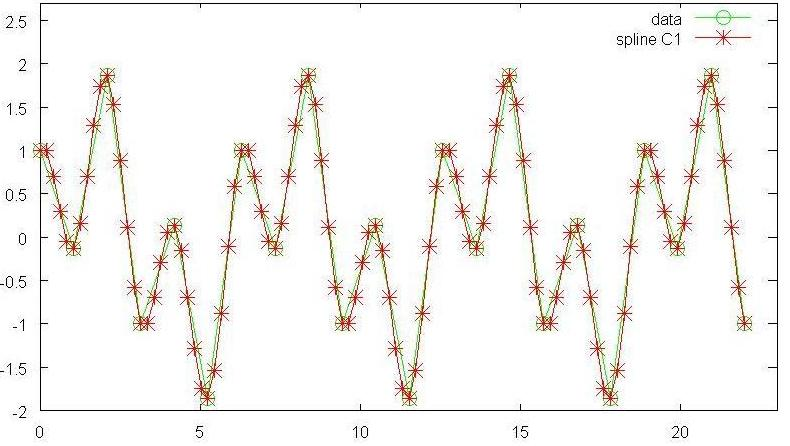
\includegraphics[width=165mm]{./img/splineC1.jpg}
	\caption{Graficul rezultat pentru fişierul de testare.}
	\label{bezi}
\end{figure}
%\end{Problem}

%----------------------------------------------------------------------------------------
%       PROBLEM 4
%----------------------------------------------------------------------------------------

\subsection{Problema 4}

Scrieţi un program OCTAVE care calculează valoarea unei funcţii într-un punct, ca rezultat al interpolării obţinute folosind funcţii spline naturale în clasă $C^2$. Programul primeşte ca parametrii de intrare: $x$ - suportul interpolării, $y$ - vectorul ordonatelor pentru valorile din suportul interpolării, $xi$ - abcisa în care se calculează valoarea funcţiei. Rezultatul programului este valoarea funcţiei în $xi$.

\textit{Soluţie:}

\octavescript{./src/SplineC2natural.m}{Interpolare cu funcţii spline naturale în clasă $C^2$.}

Pentru testarea programului puteţi folosi următoarea secvenţă:

\octavescript{./src/testsplineC2natural.m}{Fişier de testare.}

iar rezultatul este:

\begin{figure}[ht]
	\centering
	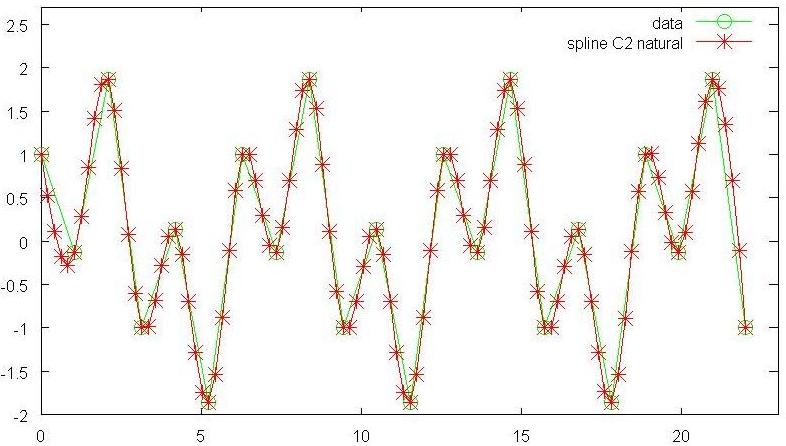
\includegraphics[width=165mm]{./img/splineC2natural.jpg}
	\caption{Graficul rezultat pentru fişierul de testare.}
	\label{bezi}
\end{figure}
%\end{Problem}

%----------------------------------------------------------------------------------------
%       PROBLEM 5
%----------------------------------------------------------------------------------------

\subsection{Problema 5}

Scrieţi o funcţie OCTAVE care să calculeze un punct aflat pe o curbă B\'{e}zier folosind algoritmului De Casteljau. Funcţia primeşte ca parametrii de intrare: $x$ - vectorul abciselor punctelor de control, $y$ - vectorul ordonatelor punctelor de control, $t$ - parametru. Rezultatul funcţiei este un punct $P$ aflat pe curba B\'{e}zier.

\textit{Soluţie:}

\octavescript{./src/Casteljau.m}{Algoritmului De Casteljau.}

Pentru testarea funcţiei anterioare puteţi folosi următoarea secvenţă care trasează o curbă B\'{e}zier folosind algoritmul De Casteljau:

\octavescript{./src/BezierCasteljau.m}{Fişier de testare.}

iar rezultatul este:

\begin{figure}[ht]
	\centering
	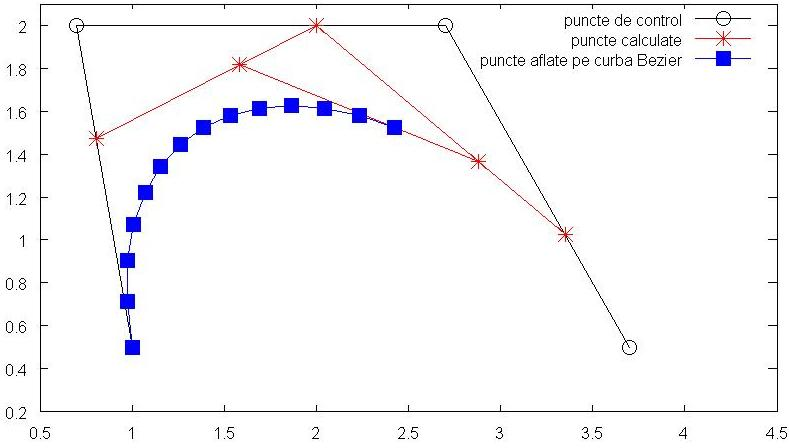
\includegraphics[width=165mm]{./img/Bezierintermed.jpg}
	\caption{Graficul intermediar rezultat pentru fişierul de testare.}
	\label{bezi}
\end{figure}

\begin{figure}[ht]
	\centering
	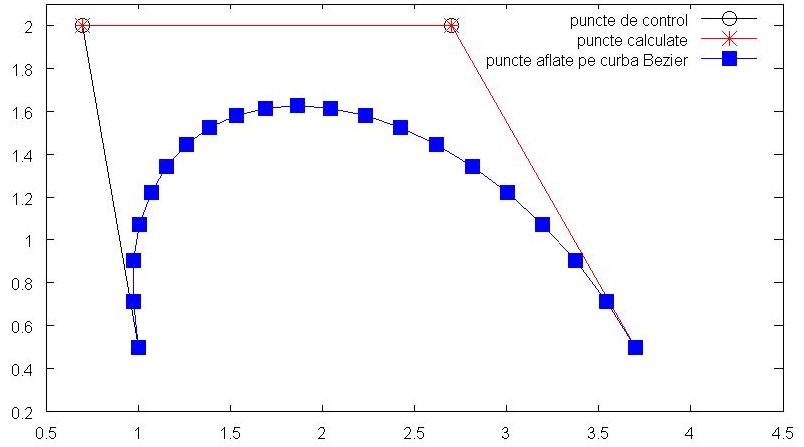
\includegraphics[width=165mm]{./img/Bezier.jpg}
	\caption{Graficul final rezultat pentru fişierul de testare.}
	\label{bezi}
\end{figure}

%\end{Problem}

\section{Probleme propuse}

%----------------------------------------------------------------------------------------
%       PROBLEM 1
%----------------------------------------------------------------------------------------

\subsection{Problema 1}

Se consideră funcţia $f$ cunoscută prin valorile:
\begin{center}
	\begin{tabular}{c || c | c | c | c}
		\textbf{x}    & \textbf{-2} & \textbf{2} & \textbf{3} & \textbf{5} \\
		\hline
		\textbf{f(x)} & \textbf{-3} & \textbf{1} & \textbf{3} & \textbf{7} \\
	\end{tabular}
\end{center}

Determinaţi valoarea funcţiei în punctul $x=1$.

%\end{Problem}

%----------------------------------------------------------------------------------------
%       PROBLEM 2
%----------------------------------------------------------------------------------------
% To have just one problem per page, simply put a \clearpage after each problem
\subsection{Problema 2}

Scrieţi un program OCTAVE care calculează valoarea unei funcţii într-un punct ca rezultat al interpolării obţinute folosind funcţii spline tensionate în clasă $C^2$. Programul primeşte ca parametrii de intrare: $x$ - suportul interpolării, $y$ - vectorul ordonatelor pentru valorile din suportul interpolării, $dy1$ - derivata funcţiei în primul punct din suportul interpolării, $dyn$ - derivata funcţiei în ultimul punct din suportul interpolării, $xi$ - abcisa în care se calculează valoarea funcţiei. Rezultatul programului este valoarea funcţiei în $xi$.

%\end{Problem}

%----------------------------------------------------------------------------------------
%       PROBLEM 3
%----------------------------------------------------------------------------------------
\subsection{Problema 3}

Se consideră funcţia $f$ cunoscută prin valorile:
\begin{center}
	\begin{tabular}{c || c | c | c}
		\textbf{x}     & \textbf{-3} & \textbf{1} & \textbf{2} \\
		\hline
		\textbf{f(x)}  & \textbf{0}  & \textbf{3} & \textbf{4} \\
		\hline
		\textbf{f'(x)} & \textbf{1}  & \textbf{2} & \textbf{3} \\
	\end{tabular}
\end{center}

Determinaţi funcţiile spline în clasa $C^1$ pentru interpolarea lui $f$.
%\end{Problem}

\end{document}
